\chapter{Etudes de cas : Patient P. , Patient E., Patiente V.}

\section{Patient P.}

\emph{``J'ai peur de l'émotion}''
\begin{itemize}
\item Patient P., de sexe masculin, 65 ans, marié, deux enfants dont un
garçon de 31 ans et une fille de 34 ans, un petit-enfant.
\item Attentes : problème avec la voix, expression bridée ( on lui a toujours
dit qu'il chantait faux), problème avec la prise de parole en public,
difficulté à se concentrer et à mémoriser, peur des émotions.
\item Anamnèse :
\end{itemize}
Traitement médical à la naissance, en raison d'une suspicion de syphilis.

Otites à répétition pendant l'enfance.

Récent bilan du médecin ORL : bonne écoute, courbe curieuse(!), conduit
auditif plus étroit que la normale.

Rien d'autres à signaler sur le plan de la santé.

Problème d'identité dû à l'absence totale de communication avec le
père 

et dû aussi à une mère dominante.

Il a été habillé en fille jusqu'à l'âge de 9 ans contre sa volonté.
Sa mère voulait une fille mais a mis au monde deux garçons.Son père
meurt aphasique et paralysé lorsque Patrice atteint ses 15 ans.

Contrairement à son frère, il arrivera à 20 ans à partir et quitter
sa mère. ``L'ambiance était horrible!''

Problèmes scolaires, arrêt en seconde mais reprise des études à 45
ans ( Bac, Master) avec obtention d'un poste supérieur.

Travail psychologique personnel important tout au long de son parcours,
avec des approches de tous genres.

A déjà suivi trois sessions Tomatis avec Voix Maternelle, sans suivi
de séances actives il y a 15 ans, dans le but d'améliorer son anglais
: résultats mitigés. 
\begin{itemize}
\item Prise en charge : séances Tomatis suivis de séances actives Tomatis
+ musicothérapie
\end{itemize}
\begin{description}
\item [{1\textdegree Test}] fin août 15, 1\textdegree session : programme
de musiques spécifiques.
\item [{2\textdegree Test}] fin de session.
\item [{3\textdegree Test}] mi-octobre, 2\textdegree{} session : programme
de musique avec filtrages partiels.
\item [{4\textdegree Test}] fin de session.
\item [{Travail}] actif journalier et intensif à domicile avec un outil
Tomatis, le Forbrain\footnote{Appareil de stimulation pour le langage, l'expression, l'apprentissage
et la mémoire,mis en point par TDSA(Tomatis Dev.) } à partir de la 2\textdegree{} session: 20mn par jour avec déclamation
et mémorisation de textes de son choix : J.J.Rousseau.
\item [{Séances}] actives 1 x par semaine , de fin octobre jusqu'à fin
décembre, pour un total de 6 séances individuelles personnalisées.
\item [{Spécificité}] : intégration de la musicothérapie
\item [{5\textdegree Test}] mi-décembre.
\item [{6\textdegree Test}] en mars 2016.
\end{description}
\begin{itemize}
\item Objectifs : 
\end{itemize}
Acceptation progressive de la voix dans son corps et pose de voix.

Acceptation de l'émotion suscitée par le son, la musique.

Acceptation de son hypersensibilité sans perte de son identité masculine.

Stimulation de l'attention, la concentration et la mémoire. 

L'aider à chercher et situer son propre``son'' intérieur, son intime
résonance.

\paragraph{Observations et description des séances : }

Le patient a réagi très favorablement à la 1\textdegree{} session
: il a été surpris d'avoir eu du plaisir à l'écoute, malgré l'appréhension
qu'il en avait, du fait d'être confronté à la musique et qui correspond
à la peur des émotions qu'elle suscite chez lui de manière générale.

Après cette 1\textdegree{} session, il a été rendre visite à sa mère,
sentiment d'apaisement.

Après la 2\textdegree{} session : Certains mots en anglais sont plus
compréhensibles, il écoute avec plaisir cette langue et la comprend
de mieux en mieux.Davantage réceptif aux sons qui l'entourent, qui
l'environnent dans la rue.

\emph{Grand travail sur la respiration, la posture, la voix }: il
est très appliqué, se sent très impliqué. 

L'humour a sa place, il a une certaine auto-dérision et les échanges
sont spontanés et joviaux.
\begin{itemize}
\item Décembre : Période de doute. Il lui semble que quelque chose bouge
et cela le met dans un inconfort certain.
\end{itemize}
Le doute est nécessaire et fait partie de son processus.

Peu à peu, il commence à accepter des\emph{ vibrations sonores sur
le corps} avec l'aide d'instruments, dont notamment le bol tibétain.

A ma suggestion de s'inscrire et de s'intéresser à faire partie d'
une chorale, il réagit catégoriquement par un refus. ``Oh! non, trop
peur de l'émotionnel! ''
\begin{itemize}
\item Fin décembre : \emph{séance très intense de musicothérapie }``pure''
où il a dû décrocher avec le verbal, pu décrocher avec le mental :
début de reconnaissance de sa grande sensibilité ; il prend conscience
qu'il refoule, repousse cet aspect féminin en lui ; sa part féminine
peut commencer à exister en lui. Ses pleurs intenses sur le violoncelle
ne sont pas une honte. Se sent un peu décontenancé.
\end{itemize}
Ouverture progressive avec encore beaucoup de peur.

En janvier 2016 : c'est la première fois qu'il s'ouvre à sa fille
et qu'il parle de son enfance et des difficultés rencontrées ; il
sent qu'il commence à lever certaines défenses : fortes émotions partagées
avec elle !
\begin{itemize}
\item La capacité à fixer son attention s'est nettement améliorée et la
sélectivité s'est ouverte. (cf.tests en annexe)
\end{itemize}
La voix se place bien, est posée; il estime que cela est plus facile
sous Oreille Electronique ( en séances) qu'avec le Forbrain; remarque
: il chante juste.
\begin{itemize}
\item Mars 2016 : s'est décidé à prendre des cours de chant et à s'inscrire
à une chorale.
\end{itemize}
Mail du patient, daté du 7 avril 2016 :

``Ce travail actif pourrait m'être très profitable et rendu possible
grâce au travail déjà effectué ensemble. Après quelques temps, j'aimerais\emph{
faire un test pour voir ce que cela aura changé dans mon écoute.}
Je vous remercie infiniment pour tout ce que vous m'avez apporté,
pour votre écoute bienveillante et chaleureuse, j'ai pris beaucoup
de plaisir à travailler avec vous et ce n'est peut-être pas fini,
j'éprouve un peu de tristesse en écrivant cela mais je sens qu'il
faut que je fasse un pas vers ce travail de la voix, vers la libération
de ma parole, quelque chose s'est ouvert et je dois avancer dans cette
direction en dépit de l'appréhension que je ressens.''

\paragraph{Constatation et remarque :}
\begin{itemize}
\item Le but serait d'accepter l'émotion et de pouvoir pleinement la contrôler. 
\item Nous estimons que le patient a fait un grand travail et son initiative
de s'inscrire à une chorale ainsi que celle de prendre des cours de
chant en sont en quelque sorte la preuve. Mais ira-t-il jusqu'au bout
de cette décision ? 
\item P. en avait conscience : son travail en profondeur n'a été qu'effleuré.
Il reste peut-être juste au seuil. Une 3\textdegree{} session? Un
suivi d'actif ? Il préfère se lancer dans des études de philosophie
et de leur donner la priorité. 
\item La confrontation avec l'émotion reste difficile pour lui mais il aurait
été intéressant, enrichissant à ce stade, ayant franchi toutes ces
étapes, de bénéficier de la musicothérapie. Profiter d'en faire l'expérience
, dans un cadre sécurisé, un espace libre, sans jugement, pourrait
lui être profitable lorqu'il sentira le moment précis où il osera
en faire le pas. Peut-être aussi ou certainement, le temps, associé
à toute cette démarche, fera-t-il simplement son travail...
\item Rencontre en décembre 2016 : Il s'est inscrit à un chorale et commence
à prendre des cours privés de chant.
\end{itemize}
P. avait besoin d'un cadre rationnel avec une procédure précise proposée
par la Méthode Tomatis. De par ce fait, elle était douce et sécurisante
pour lui et peut être ainsi considérée comme une 1\textdegree{} étape
dans un processus de transformation. Il était tout à fait perceptible
que l'espace proposé par la musicothérapie n'était pas adéquat de
prime abord. A chaque intervention purement musicothérapeutique( sans
instrument Tomatis), en phase active, P. s'étonnait, se laissait surprendre,
guider et interpeller mais finalement se retirait. Il était là, était
d'accord d'aborder certaines problématiques par la musique à travers
un matériel approprié mais pas en s'exposant de plein fouet. C'était
la solution qui lui convenait le mieux.

La musicothérapie va très vite, elle touche profondément car elle
manie le son tel un scalpel, rapide et incisif dans l'émotionnel.

\section{Patient E.}

``\emph{La musique me met face à mes problèmes}''
\begin{itemize}
\item Problèmes : Stress post-traumatique, troubles anxieux, hypersensibilité
au bruit, angoisse.
\item Anamnèse : 
\end{itemize}
de sexe masculin. 44 ans, marié, une fille de 2 ans.
\begin{lyxlist}{00.00.0000}
\item [{Naissance}] par voie basse avec 10 jours de retard, développement
normal, bonne santé générale.
\item [{Diplômes}] universitaires, Doctorat, Master.
\item [{Langues}] français, allemand, anglais, espagnol
\item [{Accident}] violent de la route en 2006, désincarcéré, amené d'urgence
en hélicoptère, bassin fracturé, traumatisme crânien à gauche, pas
de côma,1 mois d'hôpital, 5 mois difficiles de convalescence chez
lui, associée à une rupture sentimentale.
\item [{Opérations}] hernie discale, 2 vis dans le bassin ; hernie diaphragmatique
( en 2015)
\item [{Troubles}] anxieux apparaissent brutalement fin 2010, 2011 : suivi
par un psychiatre, diverses méthodes et thérapies dont la MDR , médicaments
anti-dépresseur.
\item [{Examen}] ORL en 2015 : rien à signaler
\item [{Musique}] amateur ( avant l'accident) de musique agressive, électronique. 
\item [{Ecoute}] les voix radiophoniques chaque soir pour calmer ses angoisses
et s'endormir.
\item [{Prescripteur}] : son psychiatre
\end{lyxlist}

\paragraph{Attentes : }

Atténuation de sa sensibilité au bruit qui est source d'anxiété, symptôme
de forte angoisse, apparaissant particulièrement quand il est seul
chez lui et le soir. Hors de chez lui, dans la rue, les bruits ne
sont pas anxiogènes même si cela le dérange.

\paragraph{Prise en charge globale : Tomatis et musicothérapie}
\begin{description}
\item [{1\textdegree Test}] février, 1\textdegree session : programme de
musiques spécifiques.
\item [{2\textdegree Test}] mars, fin de 1\textdegree session. 
\item [{3\textdegree Test}] début avril, 2\textdegree{} session : programmation
personnalisée, latéralisation.
\item [{4\textdegree Test}] fin avril , fin de 2\textdegree{} session.
\item [{Séances}] actives 1 x par semaine, suivi personnalisé depuis début
mai.\emph{ }Spécificité : travail en musicothérapie\emph{ et grand
travail sur la respiration, la posture, la voix .}
\end{description}

\paragraph{Observation et description des séances :}

Le patient a peu ou presque pas réagi à la 1\textdegree{} session
: il a eu beaucoup de douleurs physiques, déjà présentes avant la
session ( dues au manque d'exercice), douleur au niveau de l'hernie
discale.

a reçu ( durant la 1\textdegree session) le refus d'un poste universitaire
qu'il convoitait beaucoup : énorme déception, démotivation, rumination.

Au 10ème jour : ``meilleure digestion de son échec professionnel'',
pensées plus positives.

L'écoute des chants grégoriens a été difficile: dans la succession
des chants, il y a des pauses ( des silences) qui ont été considérées
par le patient comme anxiogènes, entre le commencement et la fin des
chants. Irritation due à l'aspect religieux du grégorien.

A repris la méditation qu'il ne pratiquait plus depuis 2 ans en raison
du silence environnant imposé par cette pratique.

A l'impression qu'il est un peu moins sensible au bruit.

``\emph{La musique me met à nouveau en face de mes problèmes.}''
(!)

Après 2 \textdegree{} session : s'est mieux passée que la 1\textdegree session;
tolère mieux le grégorien mais sans passion.Les bruits sont de plus
en plus acceptables ; si un bruit va l'angoisser, cela durera que
quelques jours au lieu de plusieurs semaines; reste toujours à l'affût
du moindre bruit avant même qu'il y en ait. A beaucoup de douleurs
physiques ( particulièrement en cette période).

Quelques jours avant la 1\textdegree{} séance active, début mai :
fortes poussées d'anxiété, angoisse d'anticipation du bruit. Les voisins
vont déménager : feront-ils du bruit? il y a une fête : ce sera peut-être
bruyant ?

Sa propre analyse : le bruit n'est pas la cause du problème mais l'idée
même qu'il s'en fait. Anticipation irrationnelle. ``C'est usant,
insupportable.''

Il ne peut s'endormir chez lui qu'avec la sécurité de rien entendre
de l'extérieur, c'est-à-dire uniquement avec des écouteurs sous forme
d'oreillettes ou des boules kiès. Nous l'incitons à commencer à les
enlever peu à peu, à faire l'effort d'en enlever au moins un pour
s'endormir. 

\paragraph{Travail avec Tomatis :}

Nous avons maintenu le grégorien \footnote{..............} pour ses
effets sur le système neurovégétatif.

Est-ce bien indiqué de l'amener à la latéralisation ? le test nous
a donné l'indication qu'il est gaucher auditif. Il serait opportun
de l'amener à privilégier l'écoute par l'oreille droite. Le message
étant clloctéé sur l'hémisphère gauche qui analyse et ``rationalise''.
Cela lui permettrait de prendre de la distance par rapport à l'émotionnel.
C'est très délicat car il a reçu le choc accidentel sur le côté gauche
et ne semble pas prêt pour l'instant. il surprotège ce côté, par réflexe
de défense, ce qui est normal. 

Objectif : réduire l'activation de la voie courte ( archaïque) pour
favoriser la voie longue avec corticalisation de l'information. On
sait que le cortex préfrontal est en relation avec le système limbique
et particulièrement l'amygdale sur lequel il exerce un contrôle. Dans
son cas, le processus de survie semble toujours en alerte, en activité,
dû au fort choc émotionnel de l'accident. L'amygdale semble avoir
été très perturbée ; les 2 sessions suivies sont peu concluantes et
nettement insuffisantes.

Faut-il poursuivre le travail ?

L'idéal, l'objectif serait qu'il puisse accepter et  transformer l'énergie
contenue dans son symptôme.

``Lifting'' .\footnote{Alfred Tomatis (1987) \emph{L'oreille et la voix. }R. Laffont, pp.206-210 }accompagné
de chants d'oiseaux et de la nature : technique respiratoire de détente
avec perception active et écoute privilégiée des aigus, filtrages
des graves pour un univers sonore plus lumineux

\paragraph{La musicothérapie : }

E. doit retrouver confiance en lui pour pouvoir contrôler l'émotion
engendrée par l'émergence d'un son. Travail selon R.Rogers. 

L'encadrement par des exercices simples du corps, des mouvements,
des exercices ludiques de voix avec main sur la poitrine le guide
pour ressentir son corps et lâcher peu à peu la dictature de son mental.

L'émission de sa propre voix lui fait prendre conscience de son corps.
La voix est un instrument intégré et vibrant dans son corps. Il a
de la peine à écouter sa propre voix et à l'accepter.

Travail avec la technique du ``Focusing'' \footnote{\emph{Focusing, }E.Gendlin, Ed. Pocket Evolution, juin 2010 }
, technique adaptée en musicothérapie par Randy Coray\footnote{Randy Coray, musicothérapeute zürichoise, professeur à E.R.M à Genève}
. Le sens corporel donne la perception de la situation émotionnelle,
de la source de l'émotion. C'est une forme d'{}''oreille'' intérieure
à une perception qui se précise avant d'être ressentie physiquement.
Ce mouvement corporel change et amène un sens corporel différent.
L'utilisation simple de voyelles (dont parle également Robert Steiner)
permet à E. de prendre le temps d'écouter son corps, de l'entendre
résonner et peu à peu de se considérer avec plus de bienveillance.

\paragraph{Constatation : }

Cela peut paraître paradoxal de vouloir faire une thérapie axée sur
le son alors que le patient ne le supporte plus. Mais cette démarche
pourrait s'apparenter à l'homéopathie. Inoculée à doses infinitésimales,
le son peut arriver à faire émerger à nouveau cet homme dans la vie
quotidienne et l'amener à vaincre peu à peu ses craintes jugées irrationnelles.

En regardant et en comparant les tests, ici le 1\textdegree{} et le
dernier en date, nous pouvons constater qu'il n'y a pas eu d'évolution
marquante. Il semble n'avoir pas ou très peu progressé. En comparant
le travail des séances avec celui reflété par le test d'écoute, nous
pouvons nous interroger sur notre travail actif et musicothérapeutique.
Quels sont les progrès que nous avions projetés et que nous avions
peut-être cru voir pendant les séances? 

La progression est peut-être réelle et se révélera dans quelques mois.
Elle n'est peut-être pas réelle et nous pouvons le constater à l'aide
du test d'écoute. 

Ce dernier nous interpelle sur beaucoup de points et nous pouvons
poser quelques hypothèses : Est-ce, par exemple, l' utilisation systématique
de boules kiès chaque soir qui aurait freiné, empêché ou faussé l'adaptation
progressive au son ? Avec les boules kiès, on impose un repos total
aux cellules ciliées de l'oreille interne. Le silence crée une réaction
contraire avec une sursensibilité aux bruits et provoque une forme
de cycle infernal . Il y avait un double travail à l'évidence, un
de jour et un de nuit. A-t- il imposé un sur-place et réduit éventuellement
la thérapie au néant ?

Ou bien est-ce le problème lié à l'opération du diaphragme ?....
\begin{itemize}
\item Pause durant l'été 2016 et non-reprise des séances.
\end{itemize}

\section{Patiente V. }
\begin{quotation}
``\emph{La musique vient dans la chair comme un produit immatériel
qui vient travailler la zone à soigner.''{}''Je pompe de la guérison.''{}''Depuis
le début des écoutes, j'ai la sensation physique et psychique de transformation.''{}''La
musique est équilibrante et guérisseuse, ma zone anesthésiée se remet
à vivre, elle est remise en activité.'' ``Il y a comme un consentement
cellulaire.''{}''La béance s'estompe, cette partie} \emph{redevient
comme les autres. Apaisement. Consentement. Réconciliation.''}

\emph{(Une patiente, V.)}

\emph{}
\begin{figure}[tph]
%\centering{}\emph{\caption{\emph{\protect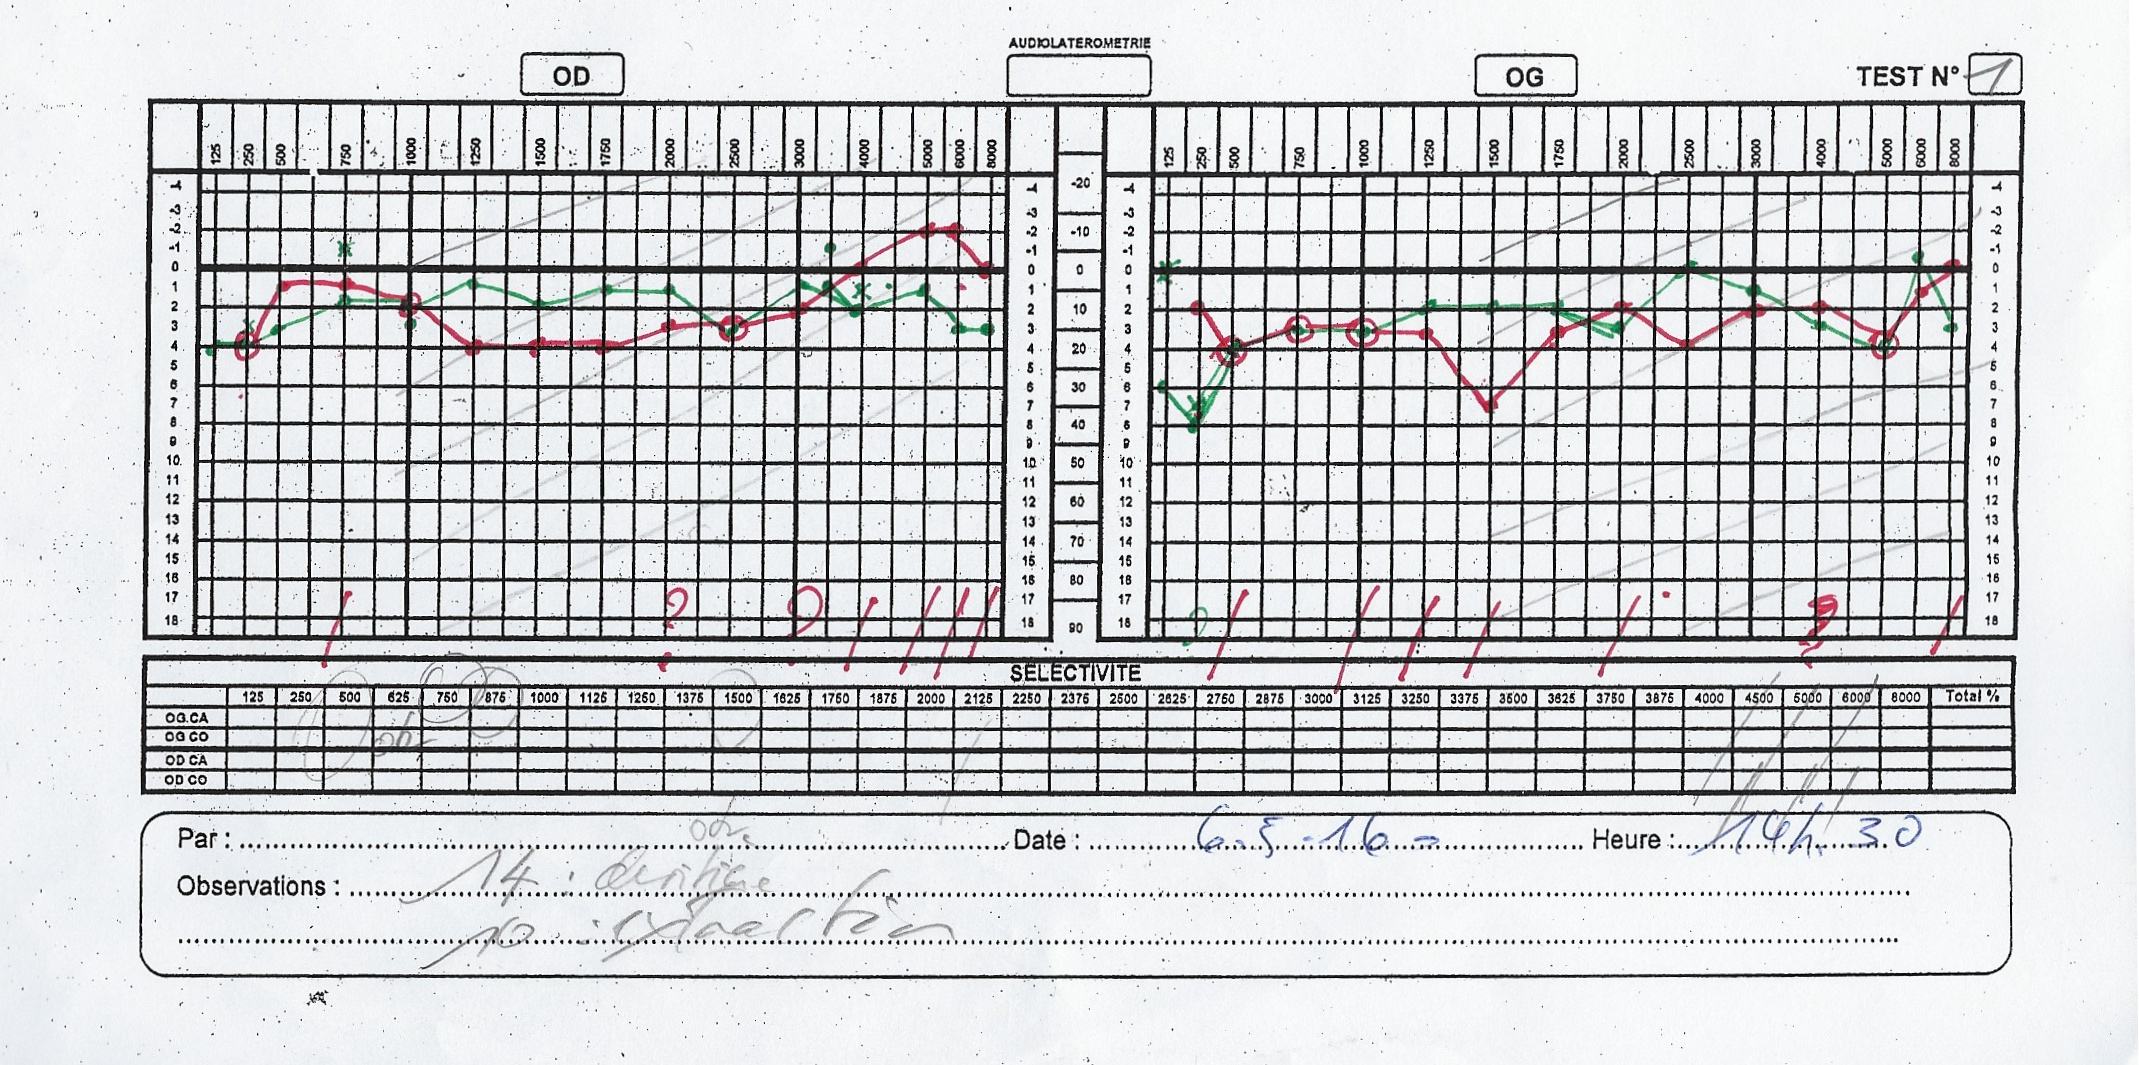
\includegraphics[scale=0.1,bb = 0 0 200 100, draft, type=eps]{PatientV1.jpg}}}
%}
\end{figure}
\end{quotation}
